%\section{ART Background Information}
%\label{sec:background}
This part provides several sections on various topics which should help to
better understand various properties and design features of ART. This part of
the document will hopefully grow over time to provide background information on
most features which are peculiar to ART.

\chapter{The Software Structure of ART}

\section{Grouping of Code into Directories}

The source structure of the toolkit groups code into a large number of
small "libraries", which are separated according to the functionality of their
contents and also according to increasing complexity. For reasons of efficiency, the small libraries are actually all compiled and linked into one large library (or framework, depending on your system). Historically, the various components actually \textit{were} separate libraries, and for reasons of code clarity, and in order to keep the overall design comprehensible, remain in the directories that used to belong to the many small component libraries of ART 1.x. An overview of the current directory groupings is shown in figure~\ref{fig:librarystructure}. Based on the library which is generated by compiling all the sources in these directories, in which practically the entire functionality of ART resides, several small-ish command line
applications like \command{artist}, \command{tonemap} or \command{impresario}, which just use the provided functionality and serve as little more than user input handlers, are built.

\begin{figure}[htbp]
\begin{center}
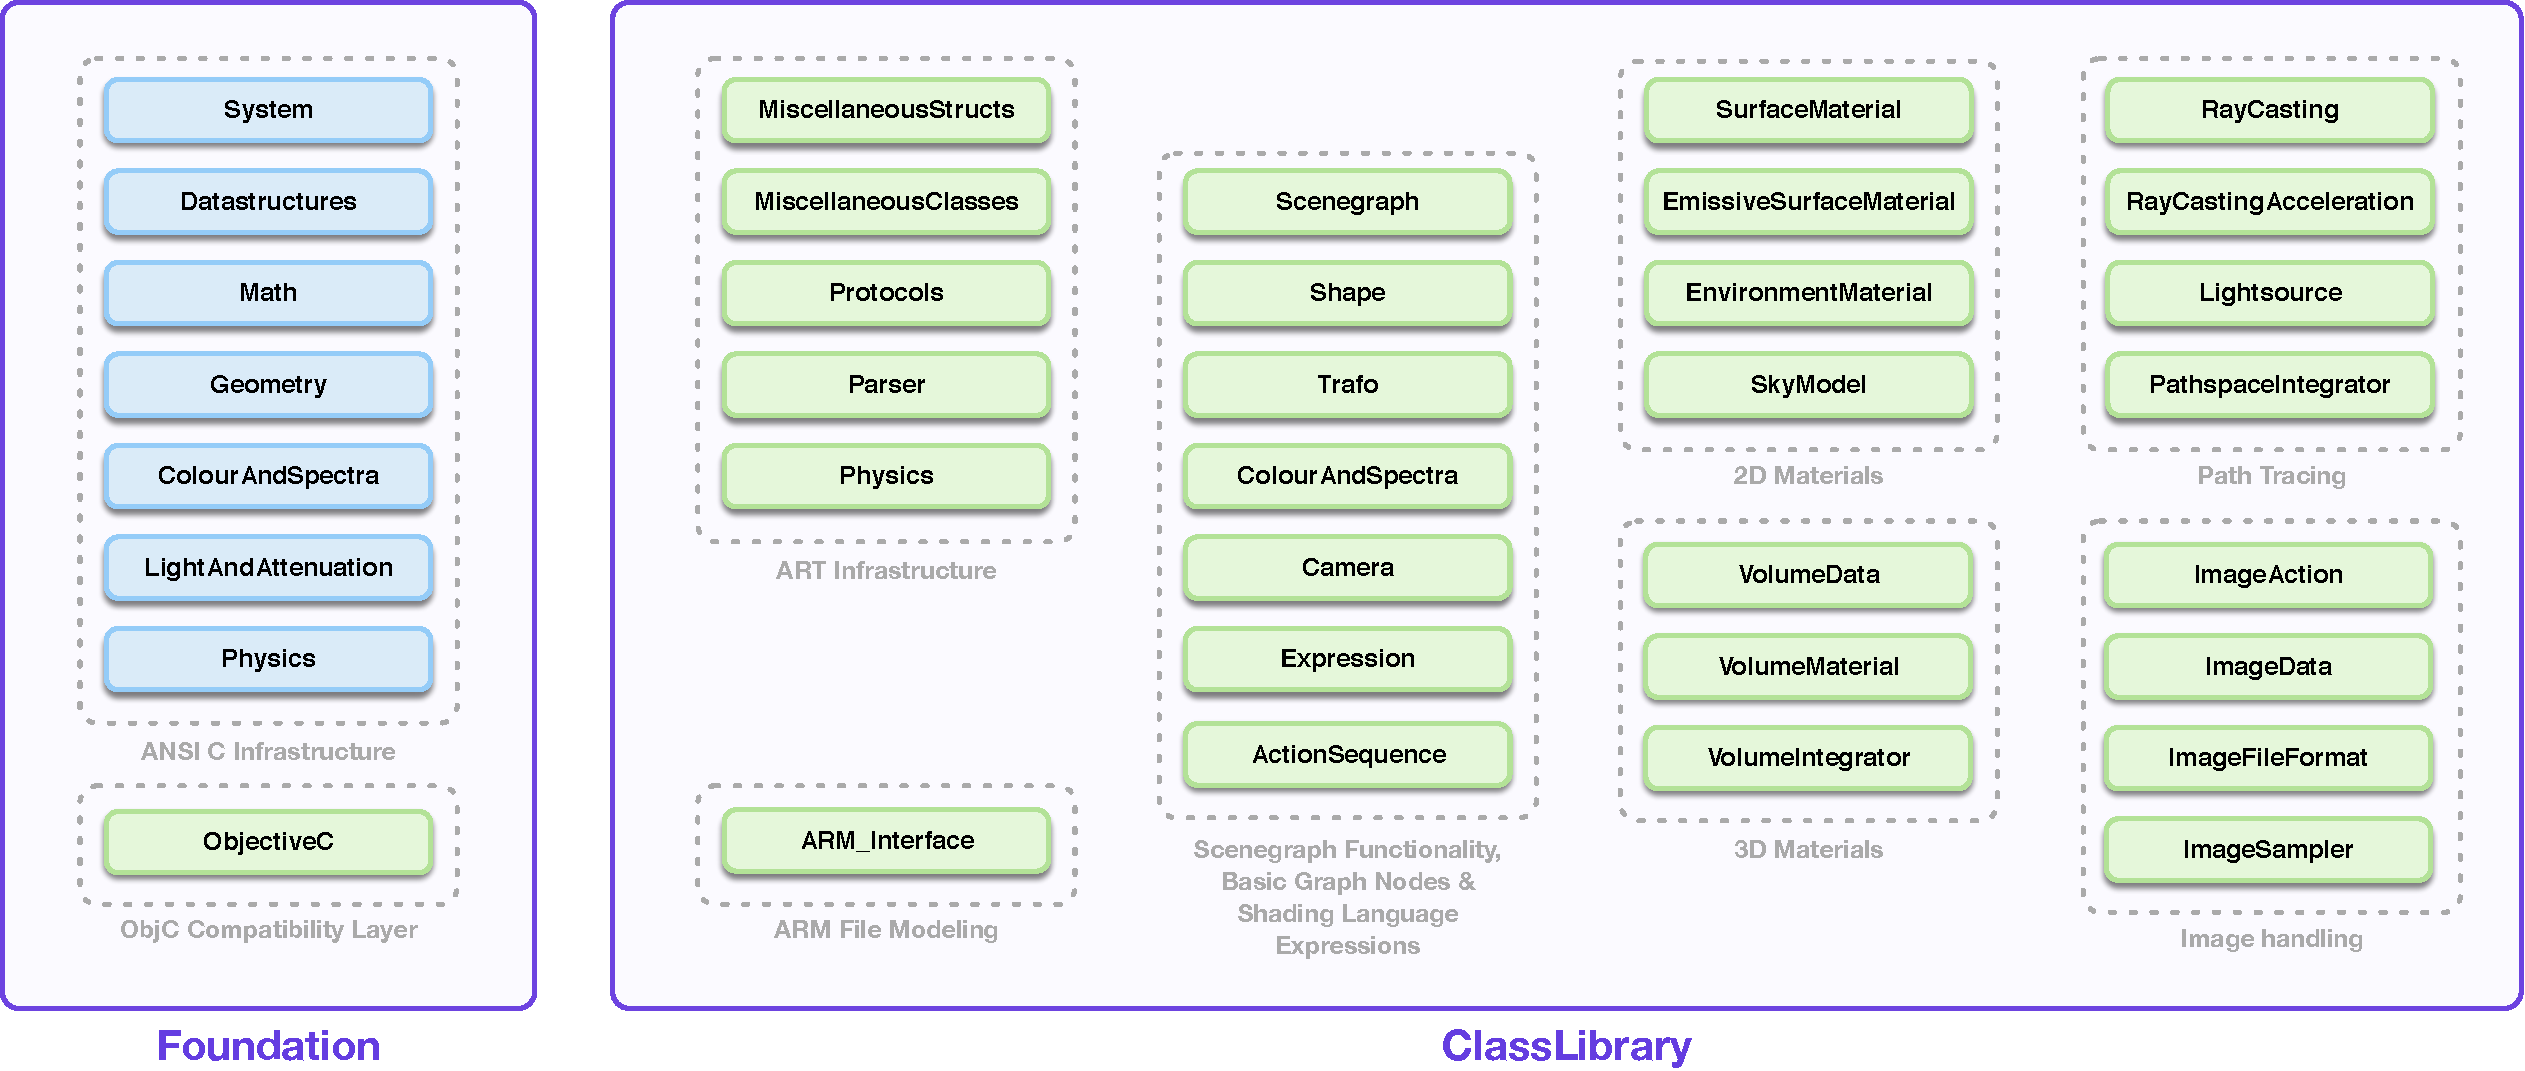
\includegraphics[width=.99\linewidth]{Images/ART_Library_Structure.pdf} 
\end{center}
\caption{
\label{fig:librarystructure} 
The overall internal structure of the ART library. Blue boxes signify sub-directories with ANSI C code, green boxes stand for Objective-C code. Note that two directory names (\source{Physics} and \source{ColourAndSpectra}) occur in both \source{Foundation} and \source{ClassLibrary}: the \source{Foundation} version contains simpler, pure ANSI C code, while the \source{ClassLibrary} directory contains classes that offer higher-level functionality. For instance, \source{ColourAndSpectra} in \source{ClassLibrary} contains scene graph nodes that deal with spectra and colours, while the 
\source{Foundation} equivalent provides low-level data types.}
\end{figure}

\subsection{Individual Source Files as \emph{ART Modules}}

Each compiled source file within ART (\ie each \source{.c}, \source{.m} or \source{.mm} file) is treated as a \emph{module}, which can have its own global state that is initialised when ART is started up, and which is destroyed in an orderly fashion when ART is shut down. To this effect, all modules contain a startup and a shutdown function, which are defined in a way that is intended to be as unobtrusive as possible. To give an example, the file \source{Foundation/System/ArTime.h} contains the following line, right after the copyright header:

\begin{verbatim}
ART_MODULE_INTERFACE(ArTime)
\end{verbatim}

This line is all that is needed for defining the appropriate function prototypes for starting and shutting down the \source{ArTime} module. In the corresponding source file \source{ArTime.c}, the following lines are also placed right at the beginning:

\begin{verbatim}
#define ART_MODULE_NAME     ArTime

#include "ArTime.h"

ART_NO_MODULE_INITIALISATION_FUNCTION_NECESSARY

ART_NO_MODULE_SHUTDOWN_FUNCTION_NECESSARY
\end{verbatim}

These lines define empty startup and shutdown functions: even if a particular source file does not need any global state, these empty functions should always be placed at the start of the source file in question. The cost of calling one empty function per source file in ART during startup is negligible, and systematically providing all modules with these functions ensures that one has module startup/shutdown infrastructure available in all parts of the system, if it were needed at a later stage in development.

Each "library" (\ie grouping of source files into thematically related source file directories, see above) has the responsibility to call the startup functions for all modules in the directory: this means that one has to manually add an appropriate line to the corresponding startup function of the library when one adds a new source file to a given directory. This is not a frequent operation, so this overhead was deemed permissible. These library startup modules are canonically named, and easy to identify: an example would be 

\begin{verbatim}
ART_Foundation_Math.[h|c]
\end{verbatim}

\subsection{Module State: the Ubiquitous Variable \source{art\_gv} }

The entire ART system is written in a way that it does not depend on any truly global variables. But as any rendering system of such size has some state associated with it, there is a ubiquitous reference within the entire codebase to something we refer to as the \emph{"ART Global Variables"}, or \source{art\_gv} for short. The data type of this variable is \source{struct ART\_GV}, and it is defined in \filename{Foundation/System/ART\_GV.h}. It is the top-level location where during module startup (see previous section), any ART module can store variable information that has to be globally accessible for a given, running instance of ART.

Apart from this struct, there are no genuine global \emph{variables} in ART, only global \emph{constants}\footnote{Some global constants, such as the \source{CRC32} tables, are actually defined as variables for technical reasons. These should never be modified, but they are usually protected by being encapsulated in their modules anyway.}. Two instances of ART can cleanly co-exist in the same memory space if each of them has their own copy of this global variable struct, and this also ensures that ART can be safely run from/as a shared library, irrespective of the memory/linkage model which is used.

There is exactly one instance of type \source{struct ART\_GV} for each running ART instance, the components of which are successively initialised during the library and module initialisation phase, and de-activated in reverse order during module shutdown. The only functions that are allowed to create the components of this struct are the canonical module startup functions discussed in the previous section, and the only ones who are allowed (and expected) to destroy its contents are the corresponding canonical module shutdown functions.

The actual data type of individual \source{art\_gv} entries is defined in each of the modules, so that no modules in ART can actually see the contents of other module \source{art\_gv} entries.

\subsection{Starting Up ART, and Shutting It Down Again}

When starting up an ART command line application, it is important that the various background sub-systems, such as the module system discussed in the preceding sections, but also the command line option handling, are started up and shut down in an orderly fashion. To make this as unobtrusive as possible, ART applications do not define their own \source{main()} functions, but instead use a template (shown here for the \source{artist} rendering application) somewhere at the end of the main source file:

\begin{verbatim}
ADVANCED_RENDERING_TOOLKIT_MAIN(artist)
\end{verbatim}

This macro defines the actual \source{main()} function called on application start-up: the predefined function takes care of all startup and shutdown issues necessary for proper ART operation. Centrepiece of this function is that it calls a user-defined actual \source{main()} function of the application, which has to have the supplied name. This function also has to have exactly the function signature seen in this example.

\begin{verbatim}
int artist(
        int        argc,
        char    ** argv,
        ART_GV   * art_gv
        )
{ ...actual code of the executable goes here... }
\end{verbatim}

Note that this signature is the same as that of a normal UNIX \source{main()} function, plus a pointer to a properly initialised \source{art\_gv} instance. This pointer is transparently passed on to all instances of Objective-C objects in the system: all classes in ART are derived from \class{ArcObject}, which contains a reference to \source{art\_gv}. As instances of \class{ArcObject} are only created via special macros which require \source{art\_gv} to be defined, the pointer is transparently passed on to all derived instances.

\section{ART as a Mixture of ANSI C and Objective-C}
\label{sect:mixingCandC}

A rather specific feature of ART which has been around since the very beginning of the 0.x series is the split of the system into a low-level ANSI C part, and a high-level Objective-C part. Unlike C++, which superficially looks a lot like C, but is actually a separate language, Objective-C is a strict superset of ANSI C, and the two can be freely intermixed and crosslinked. Back when the first versions of ART were designed by Robert F. Tobler, he carefully analysed the run-time behaviour of Objective-C, and came up with an initial distribution of data types into low level C structures, and high level ObjC classes. It is a testament to the quality of his work that this global design did not have to be modified a lot since then.

Even more than 20 years later, this split makes sense, given the properties of Objective-C: it is a powerful object-oriented language, and its advanced features such as introspection are provided via a run-time system. However, partly due to the overhead of the run-time system, one should avoid use of ObjC classes in the innermost loops of computation-intensive tasks -- at least if the instances in question might get frequently created, destroyed or modified there. In these cases, use of carefully managed ANSI C structures mani\-pulated via plain C functions make more sense, performance-wise. 

This means that in a renderer, it is reasonable to use ObjC for high-level semantic descriptions, such as the scene graph: but to also use C for low-level constructs such as points, vectors, spectra, or RGB colour values. As a consequence, the low-level libraries -- i.e. all those in \command{ART\_Foundation}, with the exception of \command{ART\_Foundation\_Objective} -- are written entirely in ANSI C99, and Objective-C is employed only \emph{above} those. However, even in high-level libraries one can find plenty of plain C structures in places where they are needed, again mostly for performance reasons.

%%%%%%%%%%%%%%%%%%%%%%%%%%%%%%%%%%%%%%%%%%%%%%%%%%%%%%%%%%%%%%%%%%%%%%%%%%%%%%%%%%%%%%%%%%%

\chapter{Memory Management in ART}
\label{sec:ARTmemorymanagement}
In this chapter, the memory management approach used on the data structure \&~class level within ART is explained. There are two main approaches to manage object persistence in non-trivial software systems:
\begin{enumerate}
\item \textbf{Garbage Collection} \\ \textit{Key advantage}: very resilient against memory-related programming errors, since no large-scale adaptation of the software is necessary. \\ \textit{Key disadvantages}: there is always a run-time penalty for the collection cycles, and if tight inner loops allocate large amounts of instances in short periods of time, memory usage spikes may result. Running the garbage collection more often to avoid such spikes reduces performance even further. Also, such usage spikes may not even be properly predictable in the first place.
\item \textbf{Reference Counting} \\ \textit{Key advantages}: memory usage never exceeds the actually needed amount, and no garbage collection cycle times are introduced. \\ \textit{Key disadvantages}: the entire software architecture has to be adapted, and it is fairly easy to make subtle and hard to find coding mistakes.
\end{enumerate}

Many years ago when the basic software design of ART 0.x was defined, reference counting was chosen as the memory management model. That was in 1996, when no robust drop-in garbage collectors existed yet, so there was little alternative to doing it this way. When the ART 2.x effort was started, it was intended to be, as far as possible, a gradual evolution and stabilisation of the ART 1.x codebase. But even fundamental design decisions like the memory management strategy were reconsidered -- especially since viable garbage collectors had become available in the meantime. 

There main reason why ART 2.x, after careful consideration, stayed with the reference counting approach of ART 1.x (albeit in an almost completely re-designed fashion) was that the potential performance penalty and memory overhead incurred by using garbage collection was deemed as being too much of a risk. In a rendering toolkit which features a shading language that is not statically "baked" into the terminal objects in a pre-processing pass (which we cannot do, as we do not break down the scene into micro-polygons before rendering), scene graph traversals can, under certain circumstances, create and almost instantly discard lots of small temporary object instances within very short timeframes. This is one usage case where garbage collection just will not work properly.

As already mentioned, the reference counting mechanisms in ART~2.x were significantly altered compared to ART~1.x. In ART~1.x, these mechanisms were not strongly formalised, somewhat varied in their semantics between different classes, and proved to be a persistent source of instability in the entire toolkit throughout its lifetime. Therefore, ART~2.x uses a fairly rigid and unified approach how object references are handled: these guidelines are what is described in the following sections of this chapter. 

\section{Design Goals of the ART Memory Management}

Those experienced in Apple MacOS application development will notice that our approach deviates to some degree from Objective-C memory management guidelines provided by Apple: ART reference counting is slightly more complicated than what MacOS does, and uses a functionality extension that is specific to ART. The extension was unfortunately necessary since ART has different goals, and faces different constraints, than the normal multi-purpose Cocoa software frameworks used for MacOS and iOS application programming. In particular, within ART object reference handling faces the following additional constraints: 
\begin{enumerate}
\item The main difference between ART and standard Cocoa/GNUStep programming is that the ability to achieve \textbf{lock-free parallelism between large numbers of rendering threads} is much more important for us than it is for normal OS~X/iOS application programming. We \textit{need} to be able to run one rendering thread per core (of which there are hopefully many), with no locking synchronisation between them taking place \textit{at all}.
\item Since descriptions of scene geometry, and their associated ray intersection acceleration structures such as kD-trees, can be very large, these many rendering threads all have to share a single copy of the scene database. By extension, this means that the rendering threads can not use retain/release operations (\ie the cornerstones of normal NSObject memory management) on that shared scene description: such operations are either not threadsafe, or -- with the OS~X/iOS runtime switched to multi-threaded mode -- use an internal semaphore protection on the reference counters that completely sends multi-thread performance down the drain.
\item Points 1 and 2 have the consequence that we have to \textbf{override the native retain/release mechanism of NSObject} with something of our own devising. The reason for this is that we still have to invoke release/retain on some objects during rendering. Since ART is designed so all these retain/release operations take place only within individual rendering threads, we do not need or want the semaphore protection that the native NSObject retain/release enforces once the system goes into multi-threaded mode.
\item During the rendering process, the presence of shading language functionality means that certain object properties, such as surface reflectance, can either be provided by actual scene database nodes (if no SL constructs are being used), or by a temporary object that contains the SL evaluation result for a particular ray-object intersection. This temporary object has to be discarded after use, while the actual scene database node must not be altered.
\item The previous point means that we need the capability to \textbf{distinguish between weak and hard object references} that are being passed to calling functions. In some cases, object references have to contain information on whether the caller should take ownership of the object it receives (in the case of a temporary node which the receiver will need to discard after use), or not (if an actual scene graph node is returned, which should not be released).
\end{enumerate}

\section{ART Memory Management - Used Data Structures}

References to object instances are normally pointers - and in ART, this is of course also the standard data type to use. Across ART, some pointers are retained by the caller, some not: which strategy applies to any given pointer should be obvious from the class definition (\ie the comments in the class definition should clearly say, for each and every pointer, to which category it belongs).

However, there are also two data types that are intended to replace pointer references to object instances in ART class definitions in all those cases where a pointer could, depending on context, be either a weak or a hard link. These types are \textbf{\filename{ArObjRef}} and \textbf{\filename{ArNodeRef}}. Apart from the typing of their contents (\filename{ArcObject} \vs \filename{ArNode} pointers), these structs are identical, and contain two fields: the pointer to the instance in question, and a field that determines whether the reference is a weak or hard link. Hard and weak references to a node instance are created by the macros \filename{HARD\_NODE\_REFERENCE(<pointer>)} and  \filename{WEAK\_NODE\_REFERENCE(<pointer>)}. The node instance pointer contained in an \filename{ArObjRef} can be accessed via \filename{ARNODEREF\_POINTER(<objref>)}.

\section{ART Memory Management - Usage Rules}

The following rules apply to all classes that are implemented within ART. (ToDo: gather the appropriate info from various header files in the source tree, where it is already provided)

%%%%%%%%%%%%%%%%%%%%%%%%%%%%%%%%%%%%%%%%%%%%%%%%%%%%%%%%%%%%%%%%%%%%%%%%%%%%%%%%%%%%%%%%%%%

\chapter{Scene File Formats}
\label{sec:scenefileformats}

In this section, we refer to all types of input files used to drive rendering jobs as "scene files", even if they only cover one particular aspect of scene appearance, or rendering behaviour. The only exception are image file formats, which are discussed in the next section.

\section{Proprietary Scene File Formats}

\begin{description}
\item[\filename{.arm}]: the native Objective-C scene file format of ART. This is the master scene file format used to drive all rendering jobs. These files are actually valid Objective-C code which constructs the scene in question, and are compiled and run in order to yield parseable \filename{.art} files: see section~\ref{sec:ARTscenefileformat} for details about how this format is read and handled by the toolkit. The extension \filename{.arm} is derived from the general prefix of things in ART (\filename{Ar...}), plus the letter \filename{m}. Normal Objective-C source files use the extension \filename{.m}, and as \filename{.arm} files contain valid Objective-C code, the combined extension makes sense.

\item[\filename{.art} / \filename{.arb}]: the internal storage format of native scene files. These are not intended to be manually edited, and their relationship to \filename{.arm} files is explained in section~\ref{sec:ARTscenefileformat}.

\item[\filename{.arh}]: ART resource header files. These are regular Objective-C header files that are used for library functions within the ART resource pool that is provided with the system. Changing the extension of these files to \filename{.h} makes no difference to their functionality, and putting resource data into regular header files would also work. The proprietary extension only serves to distinguish purely \filename{.arm}-file related headers from normal Objective-C headers.

\item[\filename{.ark}] files. These are measurement archives that usually contain spectral measurement data for reflective surfaces, and other physical measurements of materials. The archive files are intentionally human-readable, intentionally quite verbose, and the actual measurement data is stored in a format that allows direct copy and paste to Mathematica notebooks for visualisation purposes.

\end{description}

\label{sect:propsceneformats}
\section{Standard Scene File Formats}
\label{sect:stdsceneformats}

\begin{description}
\item[\filename{.ply}]: 3D mesh data. PLY is a computer file format known as the Polygon File Format or the Stanford Triangle Format. ART is capable of parsing such files, and including the geometry defined by them in native ART scenes. Support for such meshes is still not 100\% stable, unfortunately: in a few rare instances, the kD-tree builder can fail for highly complex models. Also, no mapping between vertex attributes and ART surface and material descriptors is possible yet. Currently, one can only assign one surface and one material node to the entire object described by a PLY mesh.


\end{description}

\section{Internal Handling of ARM Files}
\label{sec:ARTscenefileformat}

An at first glance perhaps slightly peculiar feature of ART is that it is actually not able to directly parse its native scene description language: the
Objective-C based \command{.arm} format. 

Instead, the native file formats that ART is actually capable of parsing are the \command{.art} and \command{.arb} formats, respectively. These two are basically the same format,
with \command{.art} being a still human-readable ASCII form of a linearised scene
graph encoding with absolute references that can easily be parsed, and
\command{.arb} being a diskspace-saving binary version of exactly the same
format. There is also a utility called \command{arb2art} available to convert
\command{.art} files to \command{.arb} format and back.

Note that \command{.art} files are -- while being intentionally
human-readable -- not really intended to be edited; although minor changes
(such as to numerical parameters of a node) can be made, any major
changes require prohibitive effort due to the absolute nature of the
references.

The \command{.arm} format is actually plain Objective-C -- the
object-oriented dialect of ANSI C in which ART itself is written. This
offers all the flexibility and power of being able to write full
C/Objective-C programs which generate the objects in the scene, and takes the
burden of maintaining such a powerful parser off the project, since
\command{gcc} or \command{llvm} are used for the translation.

Side note: by design, \command{.art} files are actually a special form of quine. The human readable form of the linearised scene graph was defined so that it is also valid Objective-C, and that it is in the right arrangement for actually even being a valid \command{.arm} file. Change the extension of any \command{.art} file back to \filename{.arm}, and you can translate it to \command{.art} form again using \command{arm2art}. Which is of course pointless, but in a certain way, also beautiful. :) Credit for this particular feature goes to Robert F. Tobler, the lead designer of ART 0.x and 1.x. We recall him enjoying himself immensely while coming up with this idea.

\subsection{\command{.arm} File Structure}
Apart from the fact that they have to be valid Objective-C, there is only one
constraint which \command{.arm} files have to fulfill in order to be usable by
the toolkit. They have to contain at least one C function with a canonical name and form:
\begin{verbatim}
ARM_MAIN_FUNCTION(<filename minus the .arm>)
{
    //   construction/initialisation of the scene object goes here
    
    return <scene_object>;   // <- return the completed scene 
                             //    object that was created
}
\end{verbatim}
so that e.g.\ the file \filename{ToyEngine.arm} has to contain a function called
\begin{verbatim}
ARM_MAIN_FUNCTION(ToyEngine)
{
    ...
}
\end{verbatim}
This "main" function has to return an \filename{ArnScene} object that defines the
overall scene structure -- see section~\ref{sec:usingart}, \emph{Using ART}, for an explanation of
its significance. Apart from this, anything goes with respect to the contents of the file. In particular, the file may include arbitrarily many other files, define functions, and do anything else that Objective-C allows. In the directory \filename{ART/Gallery}, a number of example files are provided: inspecting these will quickly give you an idea how all this works in practice.

Also, the separate "ARM Scene File Interface" guide provided in the \filename{ART/Documentation} directory gives a detailed overview of \source{.arm} file options and structure.

\subsection{Translation of \filename{.arm} to \filename{.art}}

Translation of \filename{.arm} to \filename{.art} files is simple. It is either
performed automatically in the background via a forked sub-process by \filename{artist} (or any other ART executable) whenever it senses the associated \filename{.arm} file to be newer than the corresponding \filename{.art} file, or by explicitly calling the command
\command{arm2art} as in
\begin{verbatim}
arm2art foo.arm
\end{verbatim}
or for a binary \filename{.arb} result file
\begin{verbatim}
arm2art -b foo.arm
\end{verbatim}

The actual "conversion" between \filename{.arm} and \filename{.art} is a bit of a hack, but harmless. 

First, the name of the main function of the top level \filename{.arm} file is fixed via an in-place editing pass done with \filename{sed}. This is a convenience for the end user: the requirement that the main function in a file called \filename{<filename>.arm} has to be named \filename{ARM\_MAIN\_FUNCTION(<filename>)} would make \filename{.arm} files brittle against name changes done from the command line: if you re-name an existing \filename{.arm} file, the name of the main function has to change as well. Having to do this manually every time you re-name an \filename{.arm} file would be a hassle, so the sed pass makes sure the \filename{ARM\_MAIN\_FUNCTION()} matches the filename. 

After this, the actual translation happens. In the \filename{ART\_Resources/arm2art} directory a file named \filename{ArtTranslationStub.m} is provided. What the conversion process does is the following: the scene file in question is \filename{\#included} in the stub source, the stub compiled, and the resulting executable is then run. The stub only contains a simple main routine which calls an
\filename{ArnScene}-generating function for the scene source file (the one called \filename{ARM\_MAIN\_FUNCTION(<filename minus the .arm>)}), and then simply saves this newly generated
scene graph to disk using the internal \filename{.art} format writing
routine. As last step, the translation process removes the executable which was generated to write the \filename{.art} file.


%%%%%%%%%%%%%%%%%%%%%%%%%%%%%%%%%%%%%%%%%%%%%%%%%%%%%%%%%%%%%%%%%%%%%%%%%%%%%%%%%%%%%%%%%%%

\chapter{Image File Formats used by ART}
ART uses two kinds of image formats: proprietary -- but documented -- ones for
intermediate storage of rendering results, and mainstream types for
general output.
\section{Proprietary Image File Formats}
\label{sect:propformats}
A spectral rendering system like ART has to have the capability to save the results of its
computations in a lossless intermediate format. Since ART is a rendering system that is
capable of handling spectral radiance information, and optionally also the polarisation
state of light, using existing image formats for this purpose
was unfortunately not an option. While there are multispectral some image formats out there -- mainly for use in astronomy, e.g.\ FITS -- these were designed with such different goals in mind than
fulfilling the needs of a photorealistic rendering system that it proved simpler
to design our own formats.

There are three intermediate formats specific to ART: \filename{artraw}, \filename{artcsp}
and \filename{artgsc}. The three have the following purposes: \filename{artraw} is used to
directly store all the raw information provided by the renderer which was called
by the user (which might be spectral data -- possibly including polarisation
information -- or simple colourspace values) without performing any compression, \filename{artcsp} always stores -- also uncompressed -- \filename{CIE XYZ}
colour values, while \filename{artgsc} stores single channel float images.

\begin{description}
\item[\filename{artraw}] The first format -- files with extension
    \filename{.artraw} -- has the purpose to retain all information
    available from the rendering pass, and can therefore have a wide
    variety of contents. This has to be read and interpreted by ART in any of the ISR modes it can be switched to (see section~\ref{sect:CCTs}), so the
    image format code has a crossbar-switch quality to it that makes
    it pretty specific for its purpose. An RGB renderer or tonemapper
    \eg has to be capable of interpreting a polarised spectral image
    (by converting the values to colour space and discarding the
    polarisation information), just as a polarisation-aware executable
    has to be able to read \eg \filename{CIE XYZ} image data (by
    performing an -- intrinsically problematic -- construction of
    spectra for the colour values).
    
  \item[\filename{artcsp}] The second format -- files with the
    extension \filename{.artcsp} -- is much simpler (no crossbar
    functionality -- the code is comparatively straightforward), since
    it just reads and writes floating-point colour values. It became
    necessary to develop this once we realised that prior to the availability of OpenEXR, all high-dynamic range colourspace
    formats we have been able to include in ART up to that point apparently
    performed some kind of lossy compression. Small as the error
    introduced by that was in most cases, we managed to find some
    where it made a difference. This format could be obsoleted once a
    lossless HDR format has been included in the toolkit, which now arguably is the case with OpenEXR. But then, we might just leave it in place -- never touch a running system, and \filename{artcsp}
    is used purely for internal purposes anyway. Also, in its default mode, OpenEXR tends to cut off numerically tiny result values, which has bitten us in the past.

  \item[\filename{artgsc}] The third format -- files with the
    extension \filename{.artgsc} -- is even simpler than \filename{.artcsp}: it only contains a single channel of intensity values. The reason for its existence is quite similar to why \filename{.artcsp} was created: and it is separate from \filename{.artcsp} so that a simple differentiation what kind of content what can expect is possible at the filetype level.

\end{description}
None of the three formats performs any compression, since image file size is usually not an issue for single intermediate images, and the user is free to run
\command{gzip}, \command{bzip} or some other compression tool of their choice
(which is in all probability more efficient than the kind of format-specific
lossless compression scheme we could come up with anyway) on the files if they
want to retain them.

The internals of all three formats are documented at the beginning of the
implementation files for their file format classes in:
\filename{ArfARTRAW.m}, \filename{ArfARTCSP.m} and
\filename{ArfARTGSC.m},
respectively.

\section{Standard Image File Formats}
These are used both as input formats for 2D textures (imagemaps) and as final
output formats for displayable results of rendering or tone mapping jobs. They
unfortunately differ with respect to the quality of their support in ART;
limitations are discussed along with each format.

\begin{description}
\item[Standard TIFF] Read/write implemented through Sam Leffler's TIFF
  library. Works flawlessly, and is the standard format for providing
  RGB output.
\item[JPEG] Only reading is implemented. The intention behind this was
  that lossy compression of result images is best done elsewhere, but
  that the renderer ought to be able to read JPEG imagemaps. Support is optional, and contingent on \filename{cmake} finding the JPEG library during set-up.
\item[OpenEXR] Read/write support implemented. Support is an optional feature, though: it is only present if \filename{cmake} finds the OpenEXR library during the set-up phase.
\end{description}

%%%%%%%%%%%%%%%%%%%%%%%%%%%%%%%%%%%%%%%%%%%%%%%%%%%%%%%%%%%%%%%%%%%%%%%%%%%%%%%%%%%%%%%%%%%

\chapter{Input Handling  --  File Format Handling Classes}
\label{sec:Background:InputHandling}

ART uses a modular approach to file formats. Any input data type which
can be read from file -- be that images, reflectance measurements,
scene graphs, action sequences, \ldots -- is represented by a so-called
\emph{file format handling class}. The main task of these
classes -- the names of which always begin with \class{Arf\ldots}, e.g.
\class{ArfTIFF} -- is to parse a given file, and to construct an
appropriate ART-specific representation in memory for its contents.

During application initialisation all such classes have to register
themselves with the so-called \emph{file probe} class (see the source
of an \class{Arf\ldots} class for an example of this -- the
\filename{Image} library is a good place to start looking), which is
responsible for the selection of the correct format handling class for
a given file. Amongst other things, each \class{Arf\ldots} class can
specify a list of file extensions for which it feels responsible, and
is only queried further if the filename matches one of them.

When reading a file from disc, all the programmer ever does is to request
parsing of a file which he identifies by name, and if any of the ART format
handling classes can make sense of the file contents (the file probe class holds
a contest amongst all registered format handlers to find the best one) he
receives an object instance in return:
\begin{verbatim}
object =
    parse_file(
        art_gv,
        inputFileName,
        includeLibraryPathInSearch
        );
\end{verbatim}
Due to the polymorphic nature of the parse process this \variable{object} can
theoretically be any of a wide variety of types; if the file contained a
\filename{JPEG} image, the resulting instance is actually an image
representation, while an \filename{.arm} file would result in a scene graph
object. Consequently, care has to be exercised that the correct kind of file is
parsed at the right time, and clean programming in ART would require that
objects which are read from disk are queried whether they conform to the
protocols which are needed by the calling application afterwards. 

For instance, in a scenario where the \var{object} parsed in the previous
example is expected to be an image, such a check would be achieved by the
following code: 
\begin{verbatim}
if ( [ object conformsToArProtocol: ARPROTOCOL(ArpImage) ] )
    <do whatever you intended to do>
else
    <complain / raise an exception / whatever> 
\end{verbatim}

%%%%%%%%%%%%%%%%%%%%%%%%%%%%%%%%%%%%%%%%%%%%%%%%%%%%%%%%%%%%%%%%%%%%%%%%%%%%%%%%%%%%%%%%%%%

\chapter{ART Naming Conventions}
\label{sec:Background:Naming}
For a large project like ART a consistent naming scheme for the entities which
make up the data structures within the code is crucial. Here we outline the basic
rules according to which the canonical names for structures, classes and similar
entities are derived.

\section{Data Types}
The ART libraries define a large number of data types which fall into different
categories -- C structures and several subtypes of Objective-C classes. Since
there are examples of similarly named entities which fall into different
categories, a partitioning of the project namespace according to this category
was deemed a sensible move.

Note that all data types in ART start with capital letters and are mixed case,
e.g. \class{Pnt3D}, \class{ArnSphere}  or
\class{ArnPathTracer}. Table~\ref{tab:datatypes} lists the existing
categories.

\begin{table}[htbp]
\centering
\begin{tabular}{|l|l|p{2.2cm}|p{5.7cm}|}
\hline
\textbf{\textit{Form}} 
& \textbf{\textit{Type}} 
& \textbf{\textit{Examples}} 
& \textbf{\textit{Comments, Exceptions}} \\ \hline

\class{Ar\ldots}
&
C structures and C enumerations
&
\class{ArLight} \newline
\class{ArMesh} \newline
\class{ArFileMatch}
& 
A few C structs do not follow this scheme, \eg \class{Pnt3D}. Most offenders 
   are from the \class{Graphics} library: \class{ArPnt3D} sounded too elaborate.

Sole exception in the other direction: \class{ArNode} is a node class, not a C struct (\class{ArnNode} sounds wrong) \\ \hline

\class{Arp\ldots}
& Objective-C protocols
& \class{ArpShape} \newline
\class{ArpLightsource}
& The equivalent to Java interfaces. \\ \hline

\class{Arc\ldots}
& Generic Objective-C classes
& \class{ArcRandom}
& Plain objects which are not intended to be part of scene graphs, and which are neither saved to nor
  read from file like scene graph nodes are. \\ \hline

\class{Arf\ldots}
& File format handling class
& \class{ArfTIFF} \newline
\class{ArfARTRAW}
& \class{ArcObject}-derived classes for file handling. \\ \hline

\class{Arn\ldots}
& Scene graph classes
& \class{ArnSphere} \newline
\class{ArnPathTracer}
& Nodes are the building blocks for
  scene graphs. These can be read from, and saved to, ART scene files.\\ \hline

\class{Ara\ldots}
& Scene graph attribute classes
& \class{AraTrafo3D}
& A special kind of node: all such node classes contain an indirection to an object property (shaders, trafos, \etc). Apart from this, they are normal scene graph nodes. \\ \hline

\end{tabular}
\caption{Schematic of data type naming in the ART libraries.}
\label{tab:datatypes}
\end{table}

\section{Enumeration Types}
C enumerations follow the same naming convention as C structures, namely that
they have to be of the form \class{Ar<name>}. The actual entries of the enum
are all lowercase, and their names are of the form:
\begin{verbatim}
<enum name in lowercase>_<actual value name>
\end{verbatim}
A typical example for this would be the return type of file type matching
operations:
\begin{verbatim}
typedef enum ArFileMatch
{
    arfilematch_impossible = 0,
    arfilematch_possible   = 1,
    arfilematch_exact      = 2
}
ArFileMatch;
\end{verbatim}

\chapter{Surface Materials \vs Volume Materials}
\label{sec:SurfacesVsMaterials}

In order to facilitate physics-based modelling, ART makes the usual distinction between \emph{surface materials} (\ie BRDF models), and \emph{volume materials} (which cover both material properties, and volume effects). There are a few non-standard aspects to how ART treats the relationship between those, which get explained here.

\begin{figure}[htbp]
\begin{center}
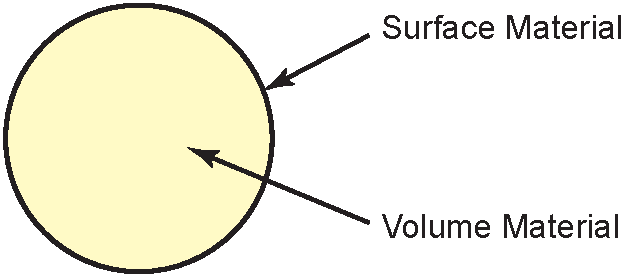
\includegraphics[width=.3\linewidth]{Images/SurfaceVsMaterial.pdf} 
\end{center}
\caption{
\label{fig:surfacevsmaterial} 
Relationship between the \source{Surface Material} and \source{Volume Material} attributes of a shape. The surface material describes the behaviour of light at the phase boundary between the shape and its surroundings. The volume material model describes both the physical properties of the volume (such as its refractive index relative to vacuum), as well as providing a mathematical model for the interaction of light with the volume inside the object.
}
\end{figure}

In other rendering systems, the mathematical models for light-surface interactions are referred to via a number of equivalent names: \emph{surface shaders}, \emph{BRDF models}, \emph{reflectance models}, and sometimes also \emph{shading models} or even \emph{illumination models}. Arguably, from a physics viewpoint, the last name in this list borders on being misleading, as these models still primarily deal with the properties of the surface in question, and not the incident illumination as such. But the expression is still common in real-time graphics.

In addition to descriptions of surface reflectance, most rendering systems also feature models for the interaction of light with volumes. These are referred to as \emph{volume shaders} or \emph{scattering models}, and are usually handled separately from the physical attributes (such as the index of refraction, or the volumetric absorption coefficient) of the objects in the scene.

In ART, we attempt to take a more unified view on this, in that each object in the scene is assumed to have a \emph{volume material} which describes its physical material properties, and, by extension, also the interaction of light with its volume. A motivation for this is that these two aspects of appearance are often tightly connected. On the other hand, the \emph{surface models} in ART are used as descriptors of light-matter interactions at phase boundaries, \ie~at the surfaces of objects. Figure~\ref{fig:surfacevsmaterial} illustrates this concept. 

This design allows for intuitive modelling insofar as surface models can take those of their input parameters which depend on the physical properties of the object they are applied to from the material description of that object, and do not have to store them themselves. An example of this are Fresnel surfaces: the main parameter of such a BRDF is the refractive index at the phase boundary. But the Fresnel surface class does not, by default, store an index of refraction, but rather uses the IOR found at the phase boundary it is being applied to instead. 

\begin{figure}[htbp]
\begin{center}
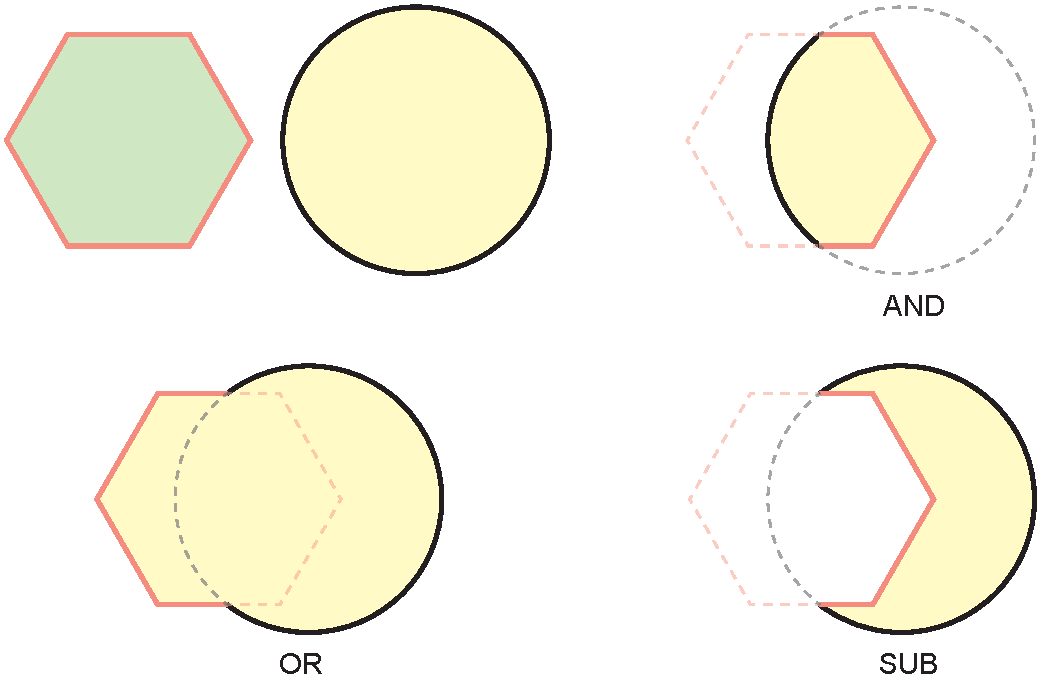
\includegraphics[width=.5\linewidth]{Images/SurfaceVsMaterialCSG.pdf} 
\end{center}
\caption{
\label{fig:surfacevsmaterialCSG} 
Behaviour of surface and volume material attributes during CSG operations. Here, it is assumed that the yellow sphere has precedence over the green hexagon, so its material is applied to the entire result. In ART, the first argument of a CSG operation has precedence over the second one, so in an \source{.arm} file, the corresponding command would \eg be \source{[sphere~sub:~hexagon]}. Note that if the red surface originally applied to the green hexagon is a BRDF which depends on volume material properties (such as a Fresnel surface material, which uses the IOR of the underlying volume material), it will use the IOR of the yellow volume material on the CSG objects! This behaviour can \eg be used to cut a piece from a glass sphere painted with opaque paint, so that one sees the glass inside again.
}
\end{figure}


From a modelling perspective, these are arguably fairly intuitive semantics for describing objects that have volume: if an object is considered to be made of glass, it has to have a glass material that, apart from storing the index of refraction of the particular type of glass used, also defines how light is attenuated inside the object (\ie also stores the transmission colour of the glass). And if the BRDF which is applied to this object needs to make use of some of this information such as the IOR, the surface model queries the material attribute for this data. 

However, an opaque BRDF which ignores the material properties can still be applied to such a glass object -- semantically, this would correspond to a glass object \eg being painted with a layer of lacquer. Inside, the object is still made of glass, though, and if CSG operations are used to cut pieces from the sphere, the glass again becomes visible. See figure~\ref{fig:surfacevsmaterialCSG} for an illustration of CSG semantics with respect to materials and surfaces.

\chapter{Surfaces}
\label{sec:Surfaces}

In this chapter, we describe some of the the technical background of the implementation and evaluation of BRDF models in ART, and present a list of the implemented models. 

\section{Technical Background}

At the moment, this section mainly focuses on things that ART does in a non-standard way, or on those aspects of a renderer where no widely accepted solution exists, and where the particular technique used in ART is worth discussing. Therefore, this section is not a complete introduction into BRDFs and surface rendering.

\subsection{The ART BRDF Model Coordinate System}
In CG literature, BRDF models are usually defined for a local coordinate system with normalised vectors of unit length that all point away from the location at which the BRDF is evaluated, and that have certain canonical names. A graphical overview of this notation is shown in figure~\ref{fig:LiteratureSurfaceCoordinateSystem}.

\begin{figure}[htbp]\centering
  \setlength{\unitlength}{2mm}
  \begin{picture}(25,10)(-10,0)
      \put(-10,0){\line(1,0){20}} % baseline
      \put(0,0){\vector(0,1){10}}     \put(0,10){$\vec{N}$} % N
      \put(0,0){\vector(-1,1){7.071}} \put(-7.071,7.071){$\vec{L}$} % L
      \put(0,0){\vector(1,1){7.071}}  \put(7.071,7.071){$\vec{R}$} % R
      \put(0,0){\vector(1,6){1.6}}    \put(1.6,9.87){$\vec{H}$} % H
      \put(0,0){\vector(2,1){8.944}}  \put(8.944,4.472){$\vec{V}$} % V
    \end{picture}
\begin{tabular}[b]{lll}
$\vec{n}$        &$\vec{N}$& surface normal \\
$\vec{\omega_o}$ &$\vec{V},\vec{E}$& outgoing direction (``eye'', ``view'') \\
$\vec{\omega_i}$ &$\vec{L}$& incoming (``light'') direction \\
$\vec{\omega_r}$ &$\vec{R}$& direction of perfectly specular reflection \\
$\vec{\omega_h}$ &$\vec{H}$& halfway vector, $\vec{\omega_h}=\frac{\vec{\omega_i}+\vec{\omega_o}}{|\vec{\omega_i}+\vec{\omega_o}|}$ 
\end{tabular}
\caption{A typical local BRDF coordinate system as used in most of CG literature. Note that all vectors point \emph{away} from the surface.}
\label{fig:LiteratureSurfaceCoordinateSystem}
\end{figure}

In contrast to this, ART BRDF models use vector directions that correspond to the ``natural'' directions of a ray-based recursive rendering algorithm, so that the incoming ray points \emph{towards} the surface. We also only refer to the involved vectors as \emph{incoming} and \emph{outgoing}. The expressions "light ray" and "eye ray" are not used, since the BRDF code might be called by a path tracer (where the incoming direction is an "eye ray"), but also by a photon tracer (where the incoming direction is a "light ray"). An overview is shown in figure~\ref{fig:ARTsurfaceCoordinateSystem}.

Note that this ignorance of which vector is the eye and which the light direction only applies to the reflectance function as such. For the construction of correct reference frames for polarising attenuation values, the BRDF code does have to know in which direction light will be traversing the evaluation location. The actual reflectance function of course has to obey the Helmholtz reciprocity principle and does not change. But based on the \source{ArPathDirection} parameter passed to all BRDF evaluations, appropriate entry and exit reference frames are constructed.

\begin{figure}[htbp]\centering
  \setlength{\unitlength}{2mm}
  \begin{picture}(25,13)(-10,0)
      \put(-10,0){\line(1,0){20}} % baseline
      \put(0,0){\vector(0,1){10}}     \put(0,10){\makebox(0,0)[br]{$\mathtt{SURFACE\_NORMAL}$}} % N
      \put(-7.071,7.071){\vector(1,-1){7.071}} \put(-7.071,7.071){$\mathtt{localI}$} % Eye!
      \put(0,0){\vector(1,1){7.071}}  \put(7.071,7.071){$\mathtt{localR}$} % R
      \put(0,0){\vector(1,6){1.6}}    \put(1.6,9.87){$\mathtt{localH}$} % H
      \put(0,0){\vector(2,1){8.9443}}  \put(8.944,4.472){$\mathtt{localO}$} % Light!
    \end{picture}
\begin{tabular}[b]{ll}
$\mathtt{SURFACE\_NORMAL}$& surface normal \\
$\mathtt{localI}$& incoming direction \\
$\mathtt{localO}$& outgoing direction \\
$\mathtt{localR}$& direction of perfectly specular reflection \\
$\mathtt{localH}$& halfway vector, $\mathtt{localH}=\frac{\mathtt{localO}-\mathtt{localI}}{|\mathtt{localO}-\mathtt{localI}|}$ 
\end{tabular}
\caption{The ART Local Surface Coordinate System. Corresponding variables are defined in all BRDF models implemented in ART. Note that the incoming direction points \emph{towards} the evaluation point. This is to avoid having to reverse the direction of the vector, which in a ray-based renderer is already available in this direction once an intersection has been computed.}
\label{fig:ARTsurfaceCoordinateSystem}
\end{figure}

\section{Surface Models Implemented in ART}

\subsection{A Note on Nomenclature}
 
    The names of the surface macros that are provided for use in ARM files follow
    a canonical naming scheme:
    
\begin{verbatim}
    <name of the model>_<BRDF type>_<additional parameters>
\end{verbatim}

    \source{<name of the model>} is straightforward: \source{LAMBERT}, \source{PHONG}, and so on.
    
    \source{<BRDF type>} is one of \source{EMITTER}, \source{REFLECTOR}, \source{REFRACTOR}, or \source{SURFACE}. The
    meaning of \source{EMITTER} is obvious, and the distinction between the remaining 
    ones (\source{REFLECTOR/REFRACTOR} \vs \source{SURFACE}) is as follows:
    
    \source{REFLECTOR} and \source{REFRACTOR} are used to distinguish between models where one
    and the same formula can be used to describe either thing happening. An example of this is
    the \source{PERFECT\_REFLECTOR} and \source{PERFECT\_REFRACTOR} pair, where a Dirac PDF is used
    for reflection and refraction, respectively. \source{REFLECTOR/REFRACTOR} surfaces
    are candidates to be combined via \source{GENERAL\_SURFACE} into compound BRDFs that
    might not be physically plausible, but at least follow mainstream CG usage of plugging several 
    simple components together to form a more complex BRDF.
    
    On the other hand, \source{SURFACE} is used for integrated models which already cover
    all aspects of a BRDF. For example, depending on the underlying material 
    node associated with the object it is assigned to, \source{SMOOTH\_FRESNEL\_SURFACE} 
    can generate both reflections and refractions, and describes the entire interaction of light with such a phase boundary. Especially the more sophisticated \source{SURFACE}s should, in general, 
    not be combined via \source{GENERAL\_SURFACE}. From a technical viewpoint, they can of course be combined, but doing so is usually even more questionable from a physics viewpoint than combining a \source{REFLECTOR} and a \source{REFRACTOR}.
    
    This distinction is not entirely clear for all cases, though. Since it is a primitive but complete model for diffuse reflectance, \source{LAMBERT\_REFLECTOR} could equally be called \source{LAMBERT\_SURFACE}. Since it is sometimes combined with a Phong component, and since there is also an emitter version of the surface, and conceivably even a refractor version of it, we on balance still opted for \source{REFLECTOR}. On the other hand, the fairly similar \source{OREN\_NAYAR\_SURFACE}, which is also sometimes used as the diffuse component of a compound BRDF, is referred to as a \source{SURFACE} because neither an emissive nor refractive version of it have been proposed so far.
 
    \source{<additional parameters>} is used to distinguish variants of a given surface
    which take additional input, such as \source{\_WITH\_MATERIAL} for surfaces which can
    maintain a material node of their own.


\subsection{List of Surface Models Currently Available in ART}

\begin{description}

\item[ArnLambertSurface] A perfectly diffuse surface that scatters with equal intensity in all directions.
\begin{verbatim}
LAMBERT_REFLECTOR(<colour>)
\end{verbatim}
The \texttt{<colour>} parameter specifies the colour of the surface. 
\item[ArnOrenNayarSurface] A diffuse microfacet model with backscattering. The microfacet distribution is modeled with a Gaussian distribution. The implementation follows \cite{conf/siggraph/OrenN94}.
\begin{verbatim}
OREN_NAYAR_SURFACE(<colour>, <sigma>)
\end{verbatim}
The \texttt{<colour>} parameter specifies the colour of the surface while \source{<sigma>} is the standard derivation of the orientation angle.  Note that the sigma parameter has to be given in radians, so that a typical invocation would \eg be

\begin{verbatim}
OREN_NAYAR_SURFACE( MUNSELL_GY_05_03, 2 DEGREES )
\end{verbatim}

\item[ArnPhongSurface] The $\cos^n$ specular reflection component of the Phong reflection model -- and only that. Use as
  part of \source{ArnGeneralSurface} combined with an
  \source{ArnLambertSurface} to get something which resembles what is commonly considered the complete Phong illumination model (\ie specular + diffuse).
\begin{verbatim}
PHONG_REFLECTOR(<colour>, <shine>)
\end{verbatim}
The \texttt{<colour>} parameter specifies the colour of the highlight, while the \texttt{<shine>} parameter is the $n$ from the $\cos^n$ formula, which defines the width of the highlight.
\item[ArnSmoothFresnelSurface] A perfectly smooth phase interface which generates a different number of BSDF samples, depending on whether the underlying material is a conductor (opaque, generates a single reflection) or a dielectric (transparent, can generate multiple BSDF samples). If the material is dielectric and not opaque, refractions are generated. The actual number of refractions depends on whether the material is isotropic/anisotropic (\ie bi-refringent) or dispersive.
\begin{verbatim}
SMOOTH_FRESNEL_SURFACE
\end{verbatim}
This surface can also store a material which is then used instead of the material associated with the object it is applied to. This allows easy modelling of \eg a silver sphere with a gold coating: if CSG operations are used to cut pieces from the sphere, the silver inside becomes visible.
\begin{verbatim}
SMOOTH_FRESNEL_SURFACE_WITH_MATERIAL(<material>)
\end{verbatim}
This BRDF model does not distinguish between stochastic and deterministic evaluation -- simply because there is no difference for a dirac pulse. 
\item[ArnTorranceSparrowSurface] The Torrance-Sparrow model (1967) with
  a Blinn (1977) microfacet distribution. Implementation based on
  \cite{975275}. However, the model as described in the book just covers the specular
  component of a surface. The model as implemented in ART takes into account that the specular
  term depends on the Fresnel term $F_r$, so there is no great
  specular reflectivity in case of near-normal ray incidence, but a
  large amount of reflectivity when the incidence angle is large, and
  the peak reflectivity is closer to the surface than the perfect
  specular direction.

  \begin{equation}
    \label{eq:TorranceSparrowART}
    fr(p, \vec{\omega_o}, \vec{\omega_i})=\frac{k_d (1-F_r(\vec{\omega_i}))}{\pi} +
    \frac{D(\vec{\omega_h})
          G(\vec{\omega_o}, \vec{\omega_i})
          F_r(\vec{\omega_i}.\vec{\omega_h})}
         {4\cos\theta_o \cos\theta_i}
  \end{equation}

Usage for metallic objects:

\begin{verbatim}
TORRANCE_SPARROW_BLINN_METALLIC_REFLECTOR(<beta>)

TORRANCE_SPARROW_BLINN_METALLIC_REFLECTOR_WITH_MATERIAL(
    <beta>,
    <material>
    )
\end{verbatim}

If a material node is supplied, the same logic as with \source{SMOOTH\_FRESNEL\_SURFACE} applies: a separate material node describes the material of a coating. 

Usage for refractive dielectric objects:
%
\begin{verbatim}
TORRANCE_SPARROW_BLINN_SURFACE(<beta>)
\end{verbatim}

Usage for objects with a dielectric layer over a base substrate:
%
\begin{verbatim}
TORRANCE_SPARROW_BLINN_LAYERED_SURFACE(
    <beta>,
    <material>
    <colour>,
    <thickness>
    )
\end{verbatim}

If the underlying material of the object this surface is applied to is a conductor, the surface is metallic. Its roughness depends on \source{<beta>}, and values close to 0 yield an (almost) perfectly specular surface. This roughness value can meaningfully go up to approximately 75 degrees.  Very low values will make the peak close to specular reflection direction, but the lobe will not shrink to a Dirac pulse, since the minimum of \source{<beta>} is clamped to 0.0001. Otherwise, if the material is dielectric, the object has the colour of the colour node, but the TS-BRDF, i.e. some energy is reflected on the surface directly and the other part enters the object and is then reflected causing Lambert reflection to emulate lacquered surfaces. In this case the parameter <colour> describes the colour of the Lambert surface. If no colour is spcified and the material is dielectric, the surface emulates sand blasted glass. 

\item[ArnGeneralSurface] With this "surface", multiple BRDF models can be combined in a linear fashion with fixed weights assigned to each of them. A typical use of this surface would be to combine an \source{ArnPhongReflector} surface with an
  \source{ArnLambertSurface}. Usage:

\begin{verbatim}
GENERAL_SURFACE(
    <weight-1>, <surface-1>,
    <weight-2>, <surface-1>,
    ..., ...,
    <weight-N>, <surface-N>,
    GENERAL_SURFACE_END
    )
\end{verbatim}

Each of the weights has to be a value greater than 0.0 and smaller than 1.0, and specifies the influence of the corresponding sub-surface on the combined surface. Use with care, since the combination of several arbitrary BRDFs is not necessarily a meaningful BRDF itself. In particular, make sure the relative weights of the individual surfaces sum to one! 

\end{description}

\chapter{Random Numbers in ART}

ART is a research system, and therefore offers a few features as switchable options which are normally either done one way or another in production systems. Random numbers are one of these areas: the functionality of the \protocol{ArpRandomGenerator}
    is a bit hybrid since it has to be a front for both "genuine" random
    generators, as well as pseudorandom sequences.

    The noticeable peculiarity which arises from this hybridization is the
    emphasis which is being put on the concept of a \emph{sequence}. While genuine
    random values are - by definition - totally uncorrelated and can be used
    in any order for any purpose, the use of sequences of pseudorandom
    numbers is typically restricted in this respect.

    An example would be that one must not use the same Halton or
    $(t,s)$ sequence for more than one decision during a singe ray traversal
    in a scene. Therefore the user has to be able to choose which generator sequence he
    wishes to use for the random value he is requesting. For genuine random
    generators, this choice is simply ignored internally.

    What makes this easier is the fact that during the rendering process, the specific sequence which is being
    requested usually does not matter as much as the fact that it is different
    from those which were used before. So as a convenience, the random
    generators are assumed to remember the sequences they have already used,
    and as their default behaviour offer to generate values from a
    "new" sequence.

    For those cases where longer sequences of random decisions of the same
    type have to be generated one can also "mark the current level" in the
    decision tree and return to it. The user still has the option of obtaining information on which sequence
    the random values he received belong to, or to explicitly generate random
    values from a specific sequence. However, these options are not very
    frequently used.

%%% Local Variables: 
%%% mode: latex
%%% TeX-master: "ARTforNewbies"
%%% End: 
